
%!TEX program = xelatex
\documentclass[letterpaper,12pt]{exam}
\usepackage{../videoNotes}
\usepackage{xcolor}
\usepackage[dvipsnames]{xcolor}
\usepackage{soul}

%\usepackage{draftwatermark}
%\SetWatermarkText{DRAFT}
%\SetWatermarkScale{1.5}
%\SetWatermarkColor{red!20}


\newcommand{\unit}{Unit 05}
\pagestyle{headandfoot}
\firstpageheader{CSC 264 \semester\ \  \unit}{}{Name: $\rule{6cm}{0.15mm}$}
\runningheader{CSC 264 \semester}{\unit}{Page \thepage\ of \numpages}
\firstpagefooter{}{}{}
\runningfooter{}{}{}

\begin{document}

%\underconstruction

\section*{\unit\_010 -- Spaghetti Bowl Programming}
\par{\fontfamily{qzc}\selectfont\textbf{Video Length 10:07}}
\begin{questions}

\begin{samepage}
    \question What was the definition of a "good programmer" prior to the middle 1960's? What problems did that definition cause?
    \vspace{5mm}
\end{samepage}

\begin{samepage}
    \question Why were most programs written before the 1970s small?
    \vspace{5mm}
\end{samepage}
\par
 \begin{samepage}
     \question Why are jmps and goto statements bad for quality programming?
     \vspace{5mm}
 \end{samepage}
 \par
  \begin{samepage}
      \question What is spaghetti bowl programming?
      \vspace{5mm}
  \end{samepage}
  \par
  \rule{0.5\textwidth}{.4pt} %End of section

\section*{\unit\_015 -- Structured Programming}
\par{\fontfamily{qzc}\selectfont\textbf{Video Length 11:45}}
\begin{samepage}
    \question What is structured programming?
    \vspace{5mm}
\end{samepage}
\par
What are the major features of structured programming? (Use your own words)
\begin{enumerate}
    \item
    \vspace{5mm}
    \item
    \vspace{5mm}
    \item
    \vspace{5mm}
    \item
\end{enumerate}
\begin{samepage}
    \question Why are if...else and while loops important to structured programming?
    \vspace{5mm}
\end{samepage}
\par
 
\begin{samepage}
    \question Can the principles of structured programming be applied to assembly language programs? Explain your answer.
    \vspace{5mm}
\end{samepage}
\par
 
\rule{0.5\textwidth}{.4pt} %End of section
%----------------------------------
\section*{\unit\_020 -- Masking}
\par{\fontfamily{qzc}\selectfont\textbf{Video Length 6:05}}
\begin{samepage}
    \question What is masking?
    \vspace{5mm}
\end{samepage}
\par
\begin{samepage}
    \question What is a bitwise AND operation?
    \vspace{5mm}
\end{samepage}
\begin{samepage}
    \question How can you tell if a binary number is even or odd?
    \vspace{5mm}
\end{samepage}
\par
\begin{samepage}
    \question What mask would you use to tell if a binary number is even or odd?
    \vspace{5mm}
\end{samepage}
\par
\begin{samepage}
    \question In the video I said that the contents of the register is "destroyed" by masking.  Explain what that means.
    \vspace{5mm}
\end{samepage}
\par

\rule{0.5\textwidth}{.4pt} %End of section
%----------------------------------
\section*{\unit\_030 -- if}
\par{\fontfamily{qzc}\selectfont\textbf{Video Length 24:26}}
\begin{samepage}
    \question Assembly language does not have an if..else structure.  Explain how I got around the lack of an "else" clause in assembly?
    \vspace{5mm}
\end{samepage}
\par

\begin{samepage}
    \question In the video I caused a link error.  How did I use the ld command to find the problem?
    \vspace{5mm}
\end{samepage}
\par
 \begin{samepage}
    \question How many jump statements (including conditional jumps did I include in the program?)
    \vspace{5mm}
\end{samepage}
\par
\section*{\unit\_040 -- if..else}
\par{\fontfamily{qzc}\selectfont\textbf{Video Length 9:35}}
\begin{samepage}
    \question How many jump statements were used when simulating an if..else block? (including conditional jumps)
    \vspace{5mm}
\end{samepage}
\par

\begin{samepage}
    \question Consider the if program from the previous video and the if..else program in this video.  Suppose you had to come in and maintain the program a year from now.  Which style would you prefer to maintain?
    \vspace{5mm}
\end{samepage}
\par
 
\rule{0.5\textwidth}{.4pt} %End of section
%----------------------------------
 \section*{\unit\_50 -- Comparisons }
 \par{\fontfamily{qzc}\selectfont\textbf{Video Length 7:06}}
 \begin{samepage}
     \question Using just jz, and jnz style of jumps, how could you determine if two numbers are equal?
     \vspace{5mm}
 \end{samepage}
 \par
 \begin{samepage}
     \question What does the cmp instruction do?
     \vspace{5mm}
 \end{samepage}
 \par
  \begin{samepage}
      \question I am not sure how to ask this as a question, but note that the cmp statement must be used with the jmp instruction.
      \vspace{5mm}
  \end{samepage}
  \par
 \rule{0.5\textwidth}{.4pt} %End of section
 %----------------------------------
\section*{\unit\_050 -- Part 2}
\par{\fontfamily{qzc}\selectfont\textbf{Video Length 7:10}}
\begin{samepage}
    \question The video shows the code for a club that requires people to be 21 or older.  Suppose it was a high-school-only club, and it only allowed in people 18 or younger.  Rewrite the parts of the code that would need to change to make it an 18 and younger club.
    \vspace{35mm}
\end{samepage}
\par
\rule{0.5\textwidth}{.4pt} %End of section
%----------------------------------





\end{questions} 
%footer
\begin{center}
    \rule{0.667\textwidth}{.8pt} %End of section
\end{center}


If you have any lingering questions or problems, please write them here or see me.
\vfill
\begin{center}
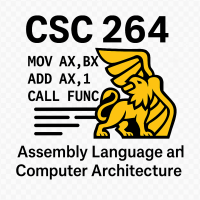
\includegraphics{../csc264Logo}
\end{center}
\end{document} 